% created on 16/11/2020
% @author : ebazan

\chapter{Landing Target Description}\label{ch:target_description}
The landing target is formed by a set of black and white circles (see Fig. \ref{fig:target_description}) that generate contours when stacked. Two of the circles ($\o_{9}$ and $\o_{10}$) have a constant diameter and form the ring that defines the target. The black circle ($\o_{11}$) is an orientation reference and has the same diameter as the smallest circle, $\o_{11}=\o_{1}$. The other circles $\o_{1}, \ldots, \o_{8}$ are coding circles.

\begin{figure}[h!]
\centering
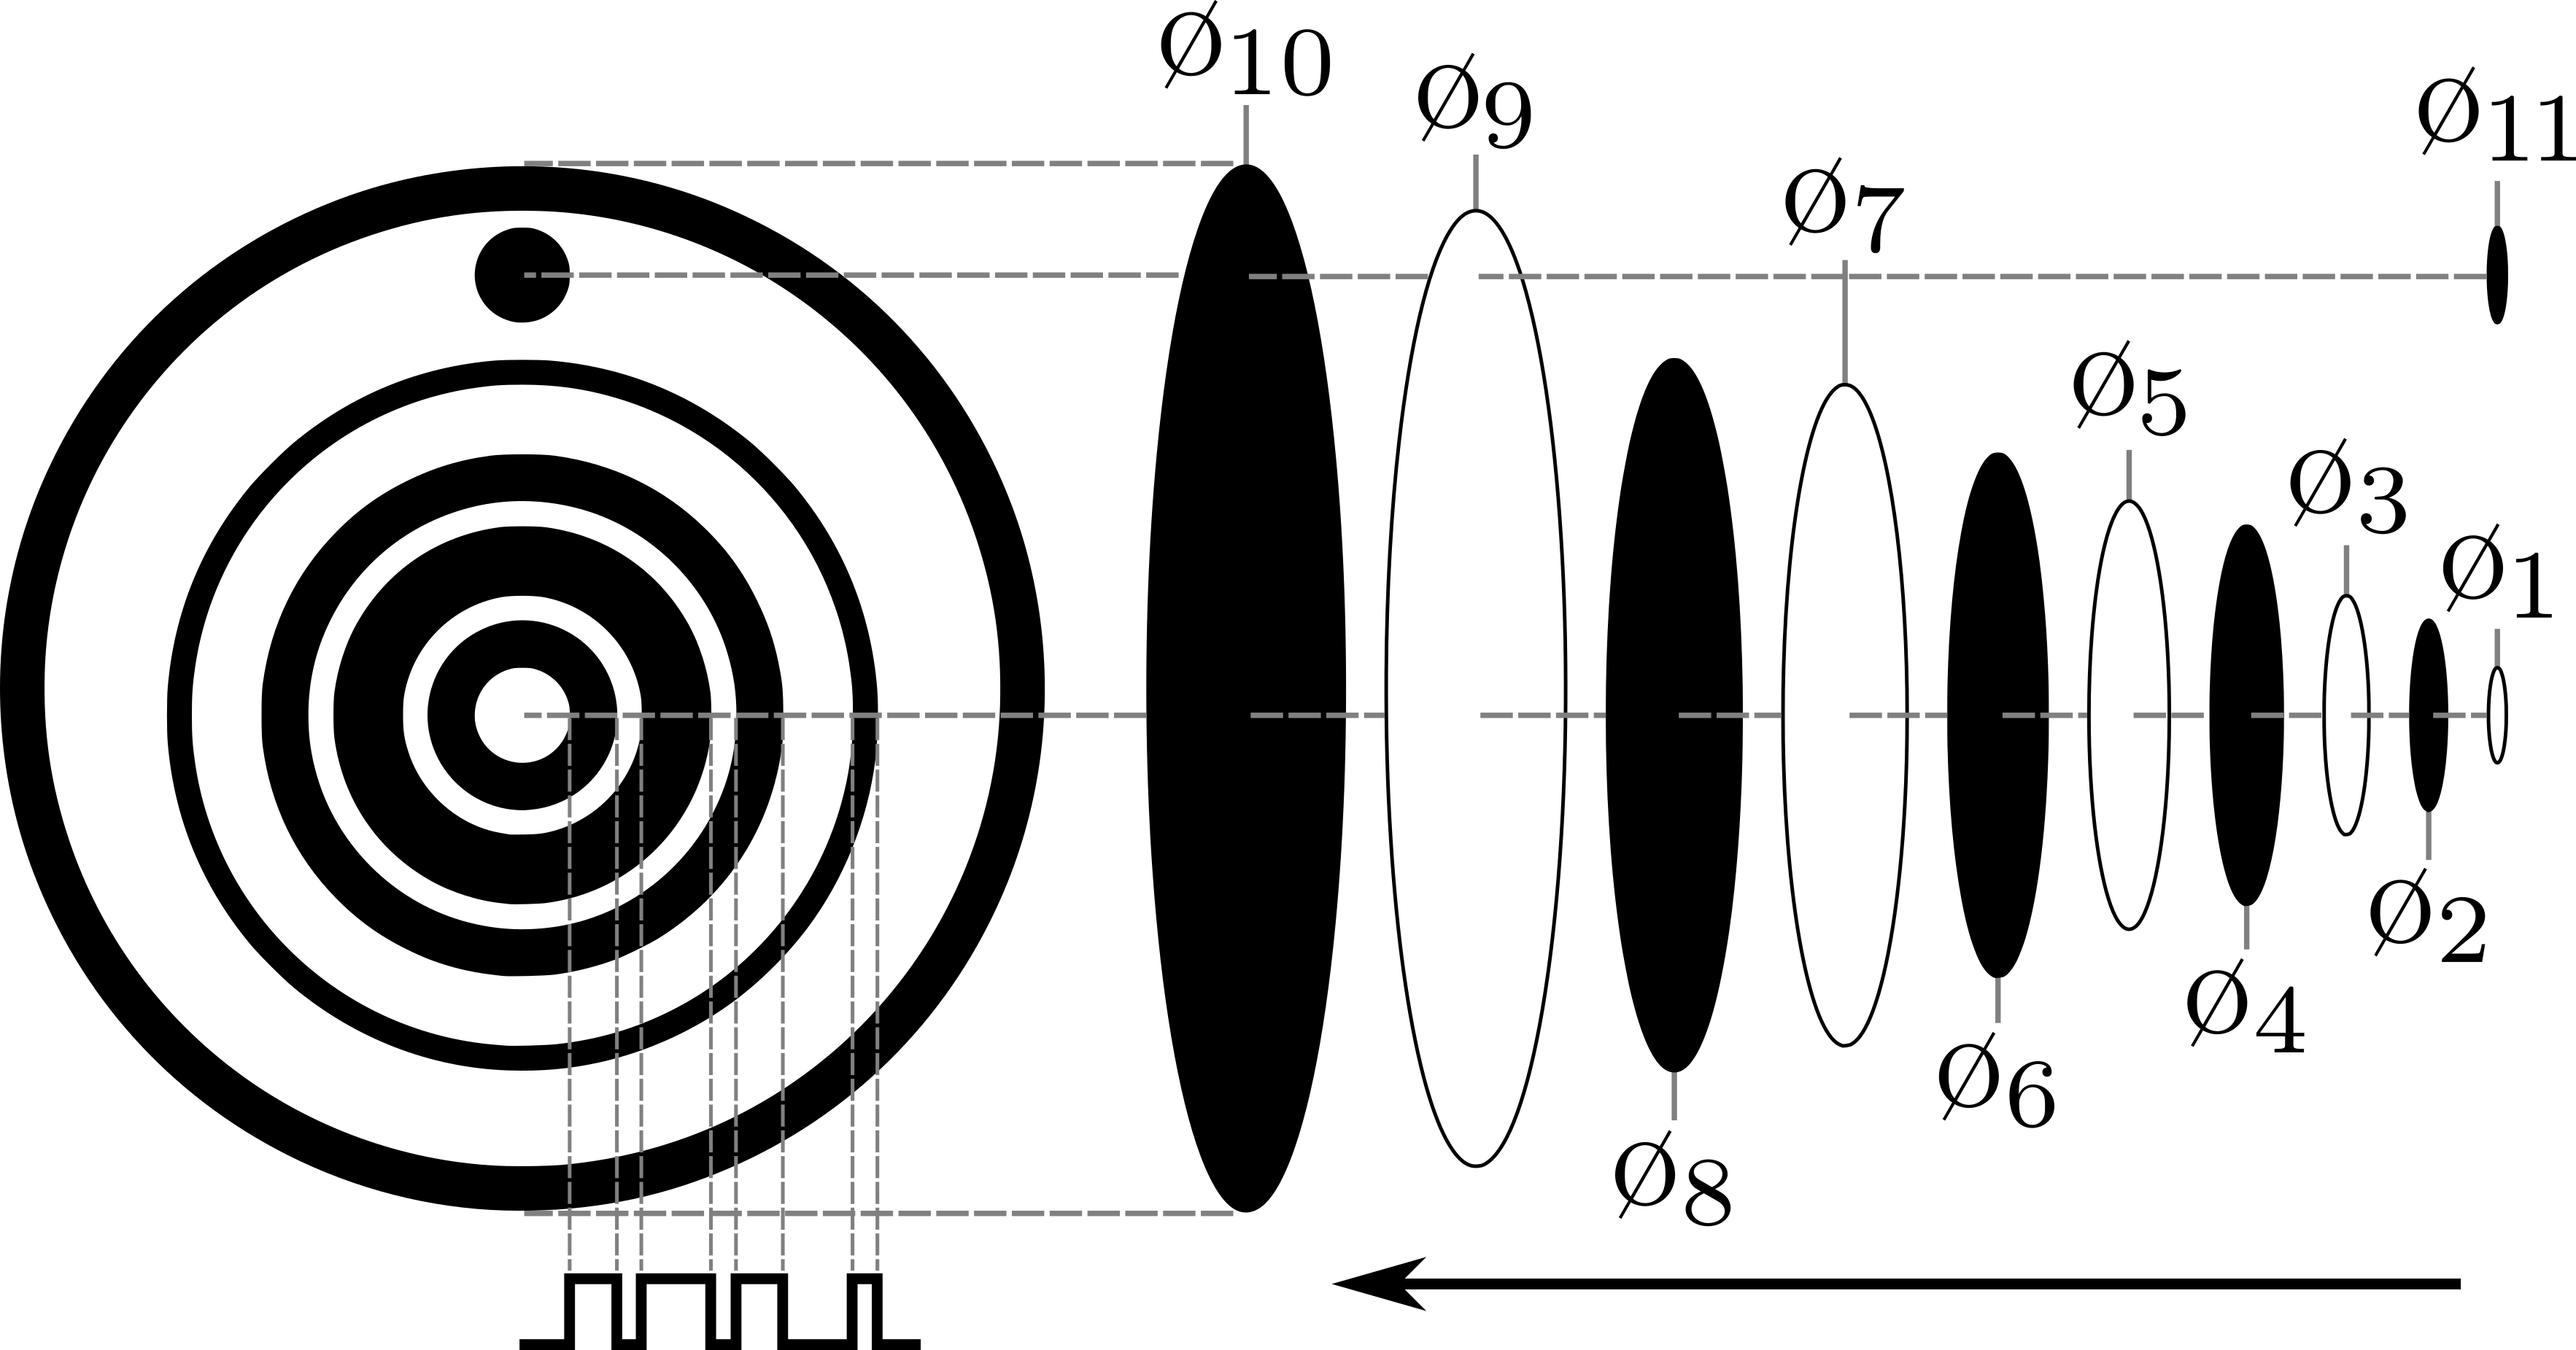
\includegraphics[width=0.8\textwidth]{target_description}
\caption{Landing target design and description}
\label{fig:target_description}
\end{figure}

\section{Landing Target ID Encoding}
Let $\O=\left( \o_{1}, \o_{2},\ldots,\o_{n}\right) $ denote the nominal diameters of the coding circles. We can set the nominal diameters, e.g., $\o_{i}=\frac{i}{n}\o_{n}$ for a target without the encoding capability. To encode a number in the target form, we modify the nominal diameters $\O$ to obtain $\O'=\left( \o_{1}', \o_{2}',\ldots,\o_{n}'\right) $ by adding/subtracting a positive constant $\Delta h$
\begin{equation}
\o_{i}'=
\begin{cases}
  \o_{i}+\Delta h, & \text{if } w_{i}=1 \\
  \o_{i}- \Delta h, & \text{otherwise }
\end{cases}
\end{equation}
and obtain a binary message  $W=[w_{1}, \dots,w_{n}]$. The message $W$ is protected from errors by Hamming error-correction code \cite{Hamming:BSTJ:1950}. It provides a set of different codewords $W= D\times M$ of size $n=k+m$, where $D$ is useful data, $ M=[I_{k}\mid 1-I_{k}]$ the generator matrix and $I_{k}$ is the $k\times k$ the identity matrix. The data vector $D$ comes from the decimal to binary conversion of the landing target ID\footnote[1]{Identification number} number. In our representation, we have experimented with $n=8$ coding circles allowing to have four rings and $n=8$ contours $\o_{1}, \ldots, \o_{8}$. This allows us to use the extended $[n,k]$ Hamming code with $k=4$ data bits and $m=4$ parity bits to generate $2^{4}=16$ landing targets.

\section{Landing Target ID Decoding.}
After the clustering stage of section \ref{subsec:clustering}, we rank by size the ellipses' major axes $\alpha_i$ by size and normalize them w.r.t. the largest value $\alpha_{10}$ to obtain %$A=(\alpha_{1}, \ldots, \alpha_{10})$  \raisebox{1mm}{$\o_{10}$}$/$\raisebox{-1mm}{$\alpha_{10}$}.
$\vec{\alpha}=  \frac{\o_{10}}{\alpha_{10}} (\alpha_{1}, \ldots, \alpha_{10})$

We compare the received and normalized axis $\vec{\alpha}$ with the nominal diameters of the coding circles $\O$ and transform them into a binary vector $\widehat{W}$;
\begin{equation}
\widehat{W}=
\begin{cases}
  1, & \text{if } \alpha_{i}-\o_{i} > 0 \\
  0, & \text{otherwise}
\end{cases} \enspace \forall i=1,\ldots, n
\end{equation}
The Hamming syndrome vector $S=\widehat{W}\times H^{T}$ (with $H=[1-I_{k}\mid I_{k}]$ as the parity-check matrix) indicates whether an error has occurred. The syndrome is a null vector $S=0$ when no error has occurred, otherwise, $S\neq 0$ and $\widehat{W}=W+E$. The element $e_{i}=0$ of the error vector $E=H^{T}-S$ indicates an error at the position $i$. The $[8,4]$ Hamming code can find up to two erroneous bits and correct one. Once the algorithm corrects the error (if there is), the vector $\widehat{W}$ is decoded by using the modulo 2 of the product $\widehat{D}=\widehat{W}\times M^{T}$. 
